As an emerging programming diagram and architecture, serverless computing is built and developed by plentiful of platforms, like AWS, Azure and Google Cloud, where the implementation is still at exploratory stage. Likewise, the rapid development of machine learning research introduces various approaches and strategies to model optimization, like hyperparameter tuning. In this section, we provide background on AWS Lambda service and hyperparameter tuning which we build upon and extend in this paper.

\subsection{AWS Lambda CPU power}

On AWS Lambda platform, every function has configuration information associated with it. One of them is the allocated memory that ranges from 128 MB to 3008 MB at increment of 64 MB. As a conventional practice, it has been announced in the official documentation~\cite{ref:lambdalimits} that AWS Lambda allocates CPU power proportional to the memory by using the same ratio as a general purpose Amazon EC2 instance type. For example, allocating 1024 MB to lambda function makes it as twice computationally powerful as allocating 512 MB. Moreover, according to AWS Lambda pricing model, the cost of lambda function is calculated by allocated memory multiplied by billed duration, namely \textit{compute charge} in GB-second.

To verify such claim, we conduct an experiment of proportional increase of CPU power along with memory. We implement and deploy a CPU-bound lambda function that multiplies two 3-D matrices. In the experiment, the host configures the function at all 46 possible allocated memory amount, triggers the function at each point and records the billed duration of execution. Figure~\ref{fig:memory} demonstrates the relationship between allocated memory (x-axis) and reciprocal of billed duration (y-axis) that represents computing power (because billed duration is inversely correlated to the CPU power). Figure ~\ref{fig:compute_charge} illustrates the relationship between memory size (x-axis) and compute charge (y-axis). We observe that the CPU power plateaued after 1600 MB. Correspondingly, the compute charge slides down from 128 MB to 1600 MB and until then increases linearly. 

Based on the above experimentation, we hypothesize the increase of CPU power is disproportional to the increase of allocated memory after a certain point. The trade-off between allocated memory and billed duration makes it possible to find a optimal (lowest) compute charge among all memory configurations. This assumption helps us build the function optimizer in the proposed framework.

\begin{figure}[t] \centering 
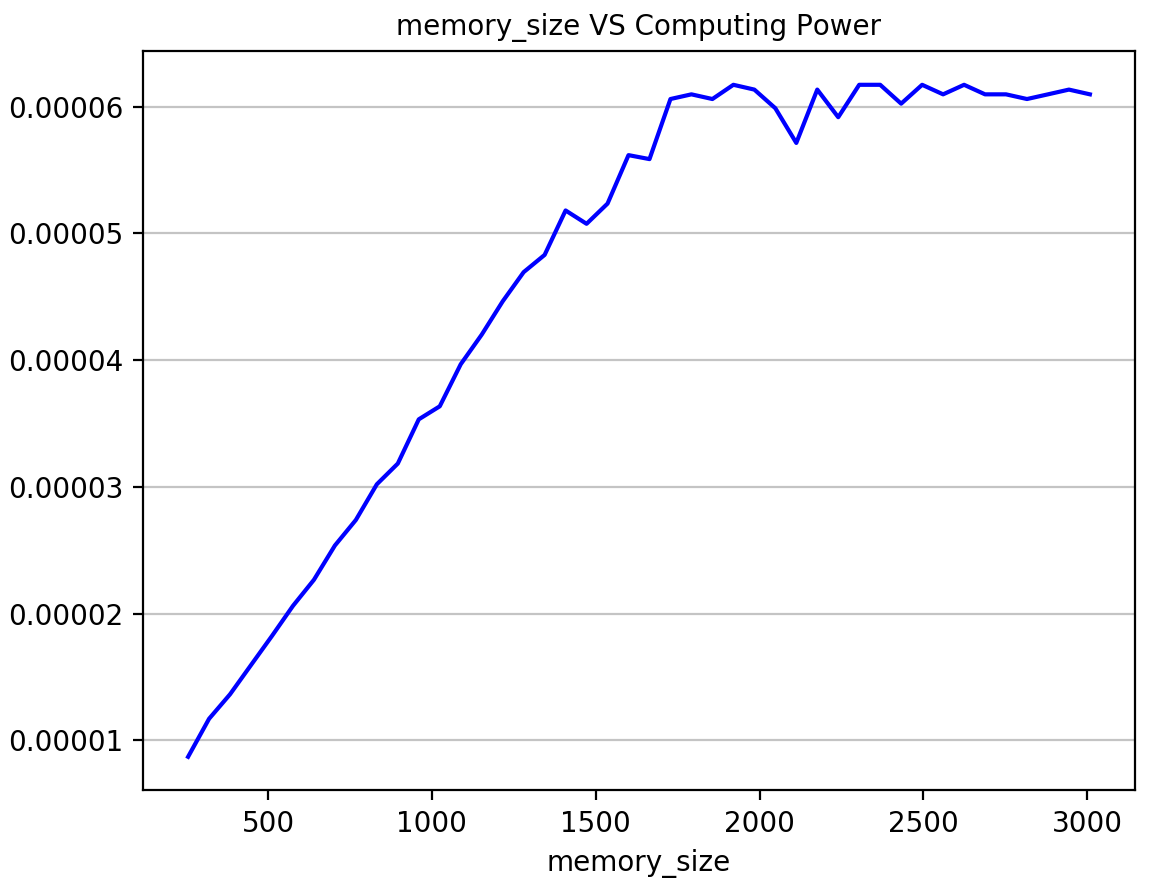
\includegraphics[scale=0.5]{memory}
\caption{The relationship between allocated memory and reciprocal of billed duration that represents the computing power.
\label{fig:memory}}
% \vspace{-0.2in}
\end{figure}

\begin{figure}[t] \centering 
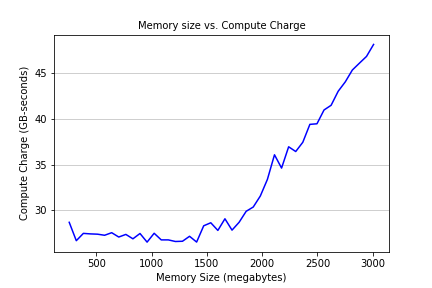
\includegraphics[scale=0.5]{compute_charge}
\caption{The relationship between allocated memory and compute charge.
\label{fig:compute_charge}}
% \vspace{-0.2in}
\end{figure}


\subsection{Hyperparameter tuning}

Hyperparameters are a set of values that put constraints on the machine learning model in order to govern the learning process. As a critical phase of model optimization, hyperparameter tuning is the searching process for the best performing parameter setting, like number of iteration or initial weights, for machine learning algorithms. Usually hyperparameter tuning is able to increase the accuracy and reduce the loss at a certain amount depending on the searching process. The exhaustive search space is the Cartesian product of all hyperparameter options and cross validation score (i.e. accuracy or mean square error) is used to evaluate different settings. Since such searching process is embarrassingly parallel, it has the potential to execute on serverless platform (i.e. AWS Lambda) in a cost-effective and low-latency fashion.